
    \documentclass[journal,twoside]{IEEEtran}
    \usepackage{cite}
\usepackage[pdftex]{graphicx}
\graphicspath{{./threestat/}}
\DeclareGraphicsExtensions{.pdf,.jpeg,.png}
\usepackage{amsmath}
\usepackage{algorithmic}
\usepackage{array}
\usepackage{url}
\usepackage{etoolbox}
\patchcmd{\thebibliography}{\section*{\refname}}{}{}{}
\patchcmd{\thebibliography}{\addcontentsline{toc}{section}{\refname}}{}{}{}

    \begin{document}
    \setcounter{page}{50}
    \title{Three Phase STATCOM using hysteresis band current control technique}
    \author{\IEEEauthorblockN{Asha Khanal, Pradip Khatri, Purushottam Khadka and Rambabu Chaudhary}\\
    \IEEEauthorblockA{Department of Electrical Engineering, Institute of Engineering, Tribhuvan University, Pulchowk, Lalitpur, Nepal}
    }


\markboth{Zerone Scholar,~Vol.~1, No.~1, November~2016}%
{Khanal \MakeLowercase{\textit{et al.}}:Three Phase STATCOM using hysteresis band current control technique}

    \maketitle
	\begin{abstract}
Reactive power compensation is very
important in power system. Most of the loads
are inductive in nature and consume reactive
power. Hence, the distribution system behaves
as the sink of reactive power. When the large
amount of lagging current flows through the
system, the system voltage goes down. In such
situation, VAR compensator brings the voltage
back to normal value. STATCOM is a FACTS
device based on VSI topology, which generally
provides superior performance characteristics
when
compared
with
conventional
compensation methods employing TSCs and
TCRs. STATCOM can supply as well as consume
reactive power. When the system needs
reactive power, it acts as a source and supplies
reactive power but when there is excess of
reactive power in the system, it acts as a sink
and consumes reactive power. This paper
presents MATLAB simulation of three phase
STATCOM. A STATCOM with the Hysteresis
band current control is developed in
MATLAB/Simulink
to
observe
their
performance.
	\end{abstract}
	\begin{IEEEkeywords}
STATCOM, Hysteresis band
current, Reactive power, PI controller

	\end{IEEEkeywords}
	\section{Introduction}
\IEEEPARstart{S}{TATCOM} is a switching converter type static
VAR generator, which generates or absorbs
reactive power without using capacitor and
inductor bank, by various switching pattern
within its converter.

\bigskip

Conventionally, capacitor banks are used to
compensate the reactive power since capacitor
draws a leading current. Power electronics
devices are gaining popularity in improving the
performance of transmission and distribution
systems. The reactive power compensation and
control have been recognized as efficient and
economic means of increasing power system
transmission capability and stability. The FACTS
devices, such as STATCOM has been introduced
more recently which employs a VSI with a fixed
DC link capacitor as a static replacement of the
synchronous condenser.

\bigskip
Functionally, the operation of the STATCOM is
similar to that of an ideal synchronous
condenser which can generate or absorb the
reactive power by varying the excitation in the
field winding. In case of STATCOM, the change in
gate signal is analogous to the change in
excitation of condenser because it causes the
change in terminal voltage of STATCOM as in the
case of condenser terminal voltage. The reactive
power in any line always flows from higher
voltage magnitude to lower voltage magnitude.
	

\section{Problem Specification}

Voltage
control
and
reactive
power
management are the two aspects of single
activity that both supports reliability and
facilitates commercial transactions across
transmission networks. In real practice, most of
the loads are inductive in nature which consume
reactive power. That means, a large amount of
lagging current drawn by the load results in
voltage sag. At low voltages, many types of
equipment perform poorly. For example: light bulb provides less illumination, and induction
motor will not operate efficiently and in some
case it may not start at all. Reactive power flow
from the generation side to the distribution side
increases transmission line losses and reduces
the power transmission capability of the transmission line. So, we use so many FACTs
controller devices to control the flow of reactive
power. Since STATCOM provides a fast response
and flexible solution to this problem, STATCOM
is the most widely use Var compensator. 



	\section{System Description}

\begin{figure}[!ht]
%\centering
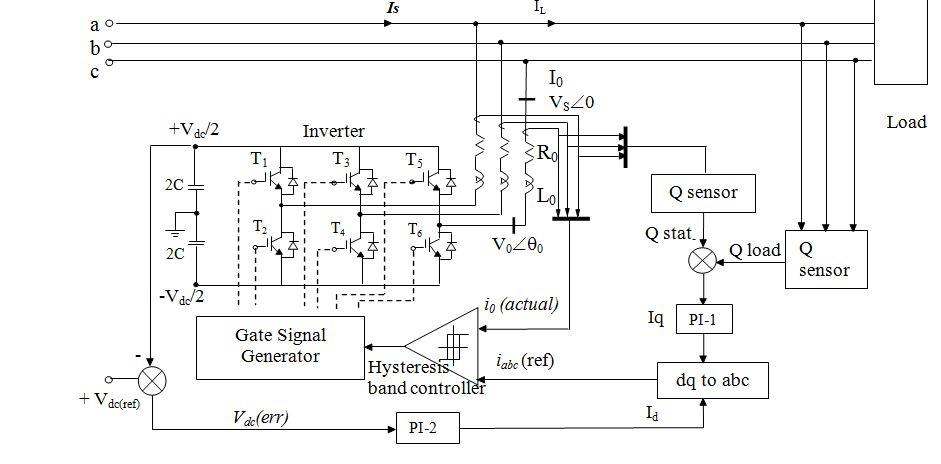
\includegraphics[width=3.7in]{1}
\caption{STATCOM System}
\label{f1}
\end{figure}

THis system includes voltage source inverter, hysteresis band controller and dc link capacitor.
The voltage source inverter consists of three
pairs of IGBTs (Insulated Gated Bipolar Gate
Transistor). Each pair consists of two IGBTs
which are switched in complementary fashion. If
the top device is on then the bottom device is off
and vice versa. Hysteresis
band controller
provides the switching signals to the IGBT by
making the actual current follow the reference
signal within the limited hysteresis band.

\bigskip
This system is designed in such a way that when
the load changes resulting the change in reactive
power, the voltage also changes( voltage
increases or decreases), it is sensed by the
voltage sensor which is compared with the reference voltage and generates an error signal
which when passed through PI controller
produces reference quadrature axis current ($I_q$).
Similarly, dc link capacitor voltage is compared
with the value of voltage that we desire it to be
constant and generates an error signal which is
fed to the PI controller produces reference direct
axis current ($I_d$). The reference direct and
quadrature axis currents when passed through
Park’s transformation (dq to abc transform)
produces reference abc phase currents. The
hysteresis band controller compares the actual
current through the STATCOM branch with the
reference currents which produces gating signal
corresponding to each leg of IGBT (one gating
signal can control both the IGBT of the same leg
since the top and bottom IGBTs are switched in complementary fashion) by comparing the
actual current of the inverter sensed by the
current sensor with upper and lower limits of
hysteresis band. This gating signal controls the
magnitude and phase of the output of the
inverter so that the inverter produces the
reactive current which compensate the reactive current drawn by the load and maintains the
voltage at load terminal. The phase is required to
compensate for the active power losses that
occur in the inverter and transformer so that the
voltage across the capacitor is maintained
constant.

\section{Matlab Simulation}
\begin{figure}[!ht]
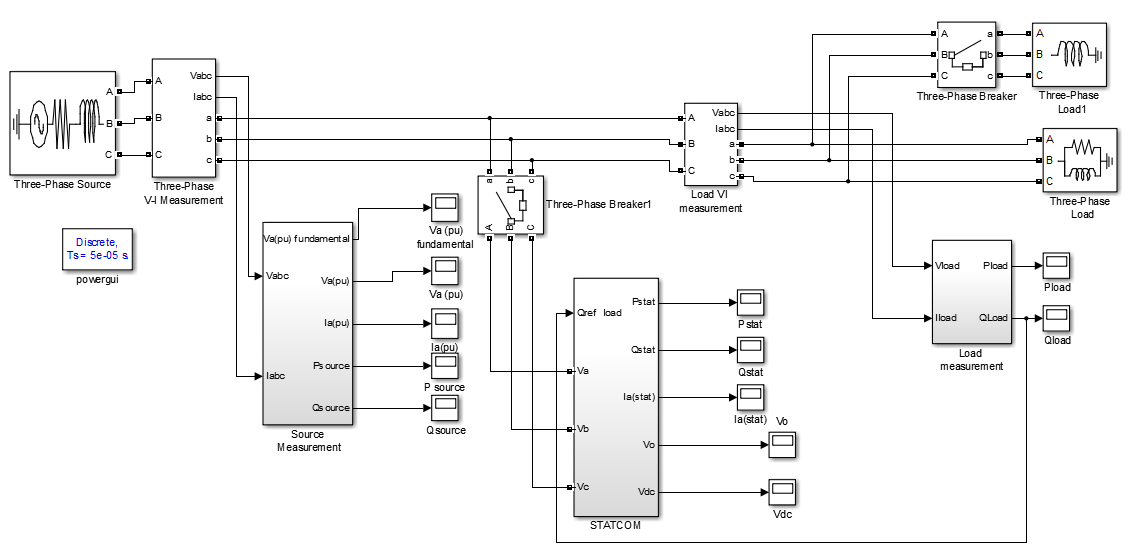
\includegraphics[width=3.5in]{2}
\caption{STATCOM model}
\label{f2}
\end{figure}

\begin{figure}[!ht]
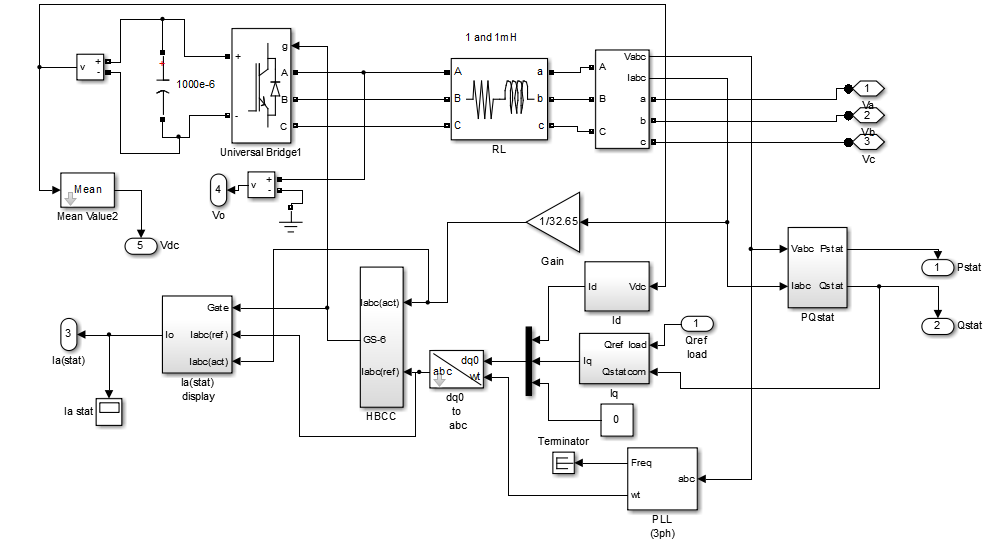
\includegraphics[width=3.7in]{3}
\caption{STATCOM Subsystem}
\label{f3}
\end{figure}
$I_d$ calculation subsystem gives the active
component of current that should flow through
STATSCOM. This block consists of a closed loop
control system with PI controller to maintain the
voltage across the dc link capacitor at reference
value. It controls the phase angle output of
STATCOM voltage. The active power loss in the
SSTATCOM branch should be supplied by the
source.
\begin{figure}[!ht]
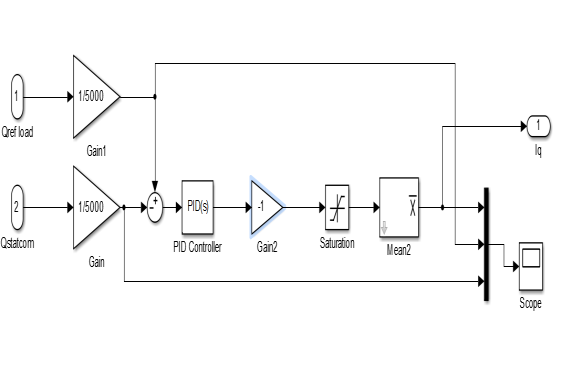
\includegraphics[width=2.9in]{4}
\caption{$I_d$ calculation subsystem}
\label{f4}
\end{figure}

If the active power through the
STATCOM branch is greater than the active
power loss, the excess of reactive power charges
the capacitor and the capacitor voltage
increases. Similarly, if the active power through
the STATCOM branch is less than the active
power loss, the deficient active power is supplied
by capacitor and the capacitor voltage
decreases. So, to maintain the value of dc link capacitor at constant value, this PI control loop
is designed. Thus, designed PI control loop will
generate the respective control signal to
maintain the capacitor voltage constant.
The reactive power demanded by the load
should be supplied by the STATCOM branch,
which is the main aim of our system.

\begin{figure}[!ht]
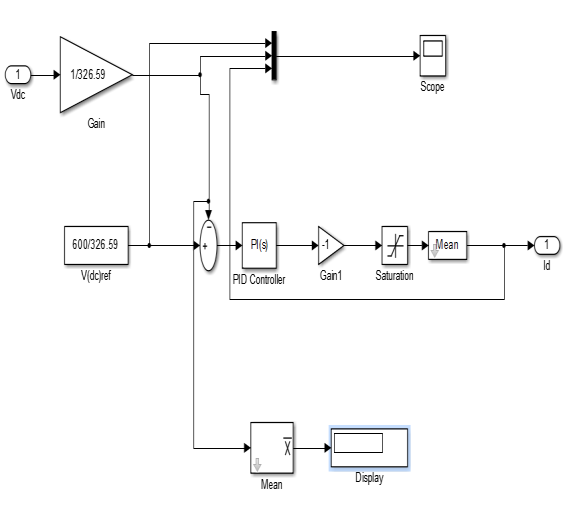
\includegraphics[width=2.9in]{5}
\caption{$I_q$ calculation subsystem}
\label{f5}
\end{figure}
 $I_q$ calculation block gives the reactive component
of current that should be supplied by the
STATCOM branch. This block consists of the
closed loop control system which compares with
the power supplied by the STATCOM with the
reactive power of the load. The error thus
obtained is passed through PI controller which
will generate the control signal to generate Iq
and compensate the reactive power.

\section{HBCC}

\begin{figure}[!ht]
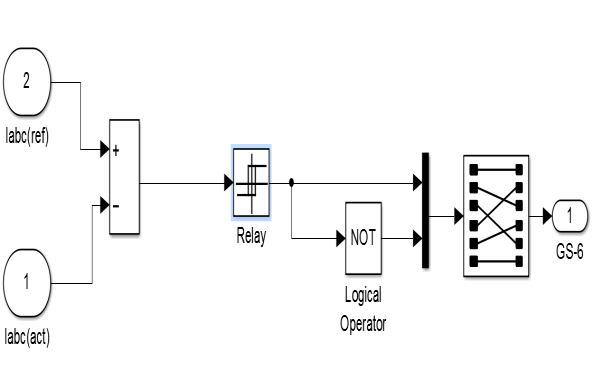
\includegraphics[width=2.5in]{6}
\caption{HBCC}
\label{f6}
\end{figure}

This is the hysteresis current control block. This
block generates the gating signals for the
inverter. In this subsystem, the reference
currents and the actual signals through the
STATCOM branch are subtracted and passed
through a relay block. The relay switches its state
when the difference tries to go beyond the two
limiting values and the gating signals are
generated. The gate signals thus obtained will
control the switching of the IGBT and thus make
the actual current within the hysteresis band.

\begin{figure}[!ht]
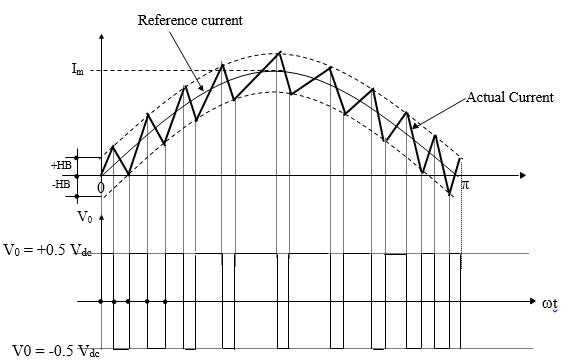
\includegraphics[width=2.5in]{7}
\caption{Actual current tracking reference current}
\label{f7}
\end{figure}

\section{dq to abc transformation}


In our system dqo to abc transformation
generates the reference signals for the
STATCOM currents. dqo to abc transformation is
also known as inverse Parks transformation.

\[
\begin{bmatrix}
u_a \\ u_b \\ u_c
\end{bmatrix}
=
  \begin{bmatrix}
    cos(\theta) & -sin(\theta) & 1\\cos(\theta-\frac{2\pi}{3}) & -sin(\theta-\frac{2\pi}{3} & 1\\ cos(\theta+\frac{2\pi}{3}) & -sin(\theta+\frac{2\pi}{3} & 1
  \end{bmatrix}
\begin{bmatrix}
u_d \\ u_q \\ u_0
\end{bmatrix}
\]

%MATRIX IN LATEX MUST SEE


\section{Rating of Different Parameters}
System voltage: 400 V\\
Dc link capacitance: 1000 uF\\
Dc link Reference voltage: 600 V\\
PI for $i_d$ loop:\\
$K_p$ =1 and $K_i$ =2\\
PI for $i_q$ loop;\\
$K_p$ = 0.1 and $K_i$ = 15\\
Hysteresis bandwidth: 5\% of reference\\
Coupling parameters\\
Inductor: 1 mH\\
Resistor: 1 ohm\\

\section{Simulation Results}

The complete MATLAB model for the simulation
of three phase STATCOM is shown in the figures 8 to 19. The horizontal axis indicates time in second and the vertical axis the respective values.


\bigskip
\begin{figure}[!ht]
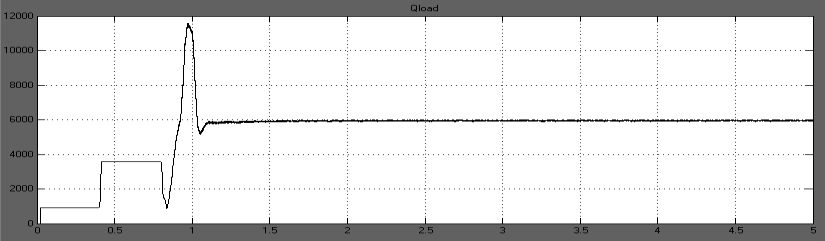
\includegraphics[width=3.5in]{a}
\caption{Reactive power consumed by load in VAR $Q_{load}(VAR)$}
\label{fa}
\end{figure}

\begin{figure}[!ht]
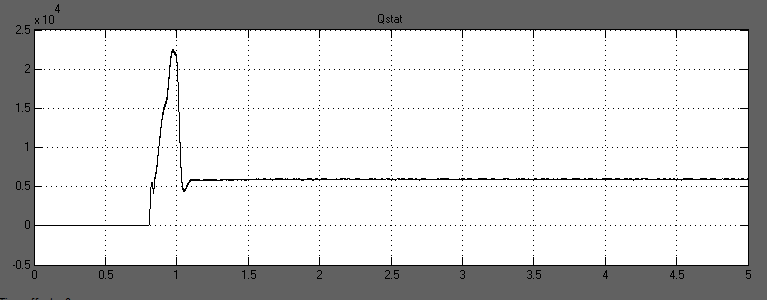
\includegraphics[width=3.5in]{b}
\caption{Reactive power consumed by STATCOM in VAR $Q_{stat}(VAR)$}
\label{fb }
\end{figure}


%Lot of Images
\begin{figure}[!ht]
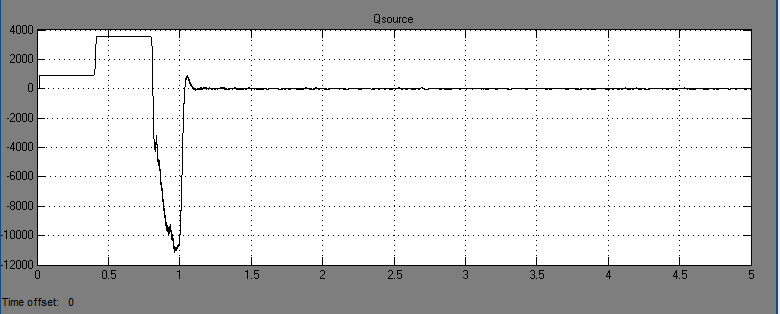
\includegraphics[width=3.5in]{c}
\caption{Reactive power supplied by source in VAR $Q_{source}(VAR)$}
\label{fc }
\end{figure}


\begin{figure}[!ht]
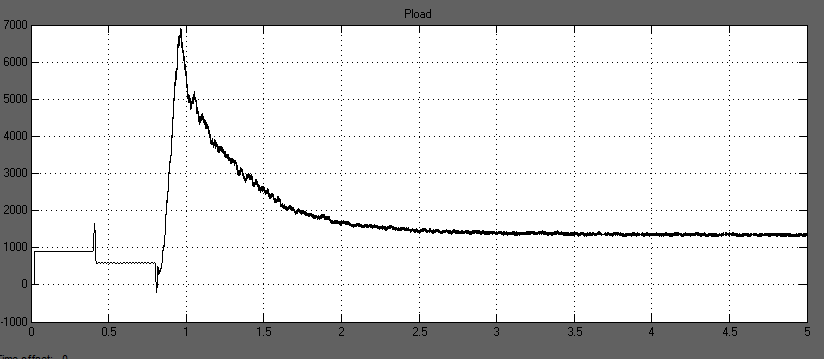
\includegraphics[width=3.5in]{d}
\caption{Active power consumed by load in watt $P_{load}(watt)$}
\label{fd }
\end{figure}

\begin{figure}[!ht]
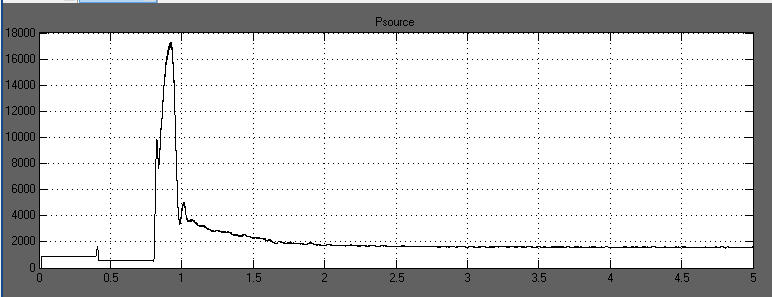
\includegraphics[width=3.5in]{e}
\caption{Active power supplied by source in watt $P_{source}(watt)$}
\label{fe }
\end{figure}


\begin{figure}[!ht]
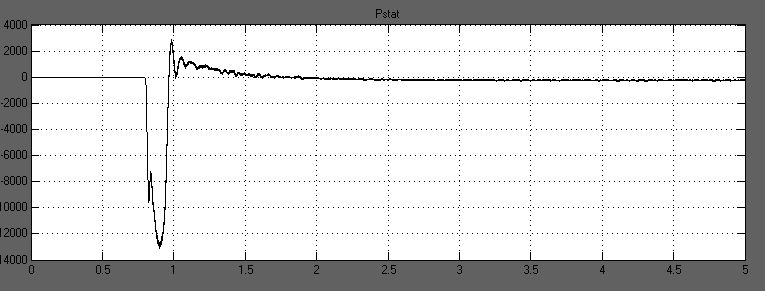
\includegraphics[width=3.5in]{f}
\caption{Active power consumed by STATCOM in watt $P_{stat}(watt)$}
\label{ff }
\end{figure}


\begin{figure}[!ht]
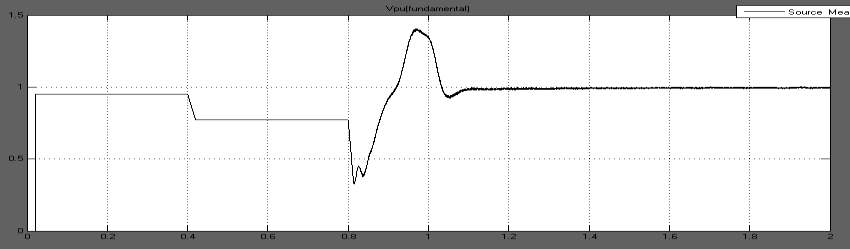
\includegraphics[width=3.5in]{g}
\caption{Fundamental component of system voltage in p.u. $V_{system}(p.u.)$}
\label{fg }
\end{figure}


\begin{figure}[!ht]
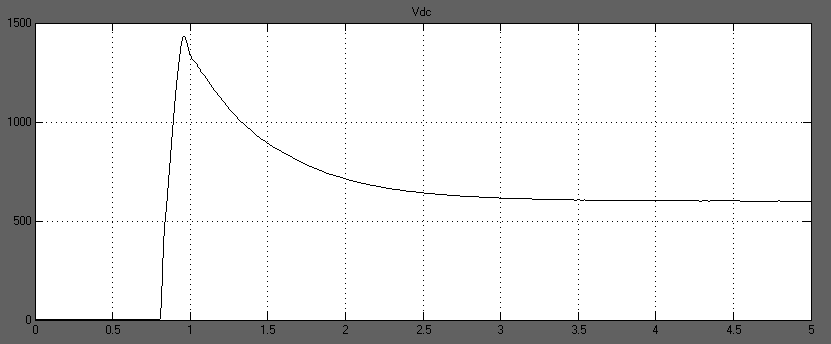
\includegraphics[width=3.5in]{h}
\caption{Voltage across dc link of capcitor in volt $V_{dc}$}
\label{fh }
\end{figure}


\begin{figure}[!ht]
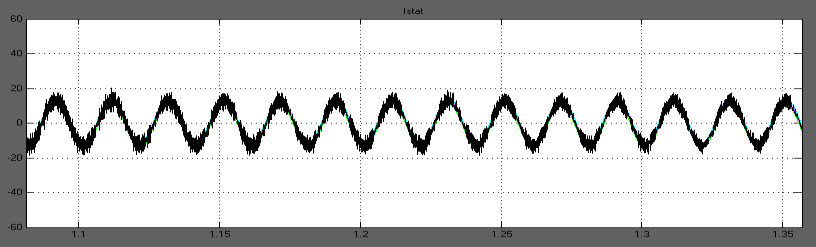
\includegraphics[width=3.5in]{i}
\caption{ Current through STATCOM branch in ampere$I_{stat}(A)$}
\label{fi }
\end{figure}


\begin{figure}[!ht]
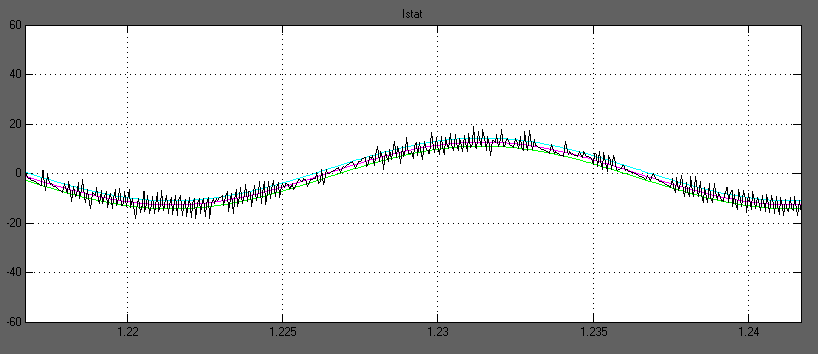
\includegraphics[width=3.5in]{j}
\caption{Magnified view of current through STATCOM branch in ampere $V_{stat}(V)$}
\label{fj }
\end{figure}


\begin{figure}[!ht]
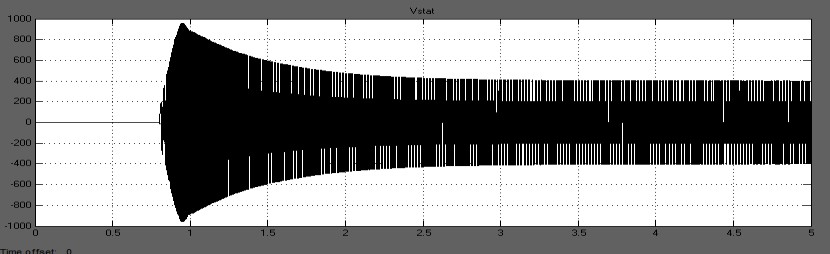
\includegraphics[width=3.5in]{k}
\caption{Output voltage of inverter in volt $V_{stat}(V)$ }
\label{fk }
\end{figure}


\begin{figure}[!ht]
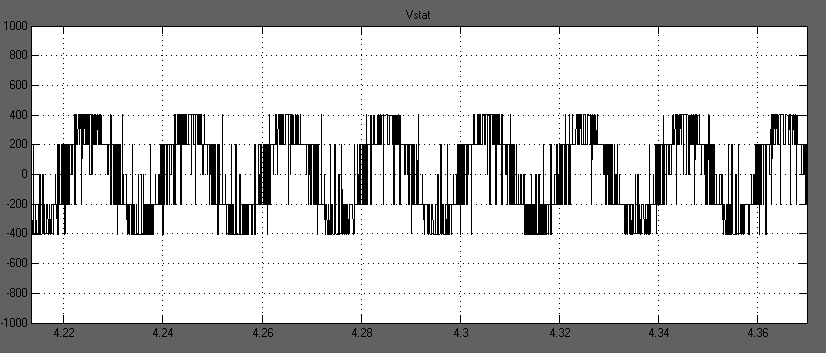
\includegraphics[width=3.5in]{l}
\caption{Magnified view of output voltage of inverter in volt $V_{stat}(V)$}
\label{fl }
\end{figure}







This model consists of three phase voltage
source with the rating of 400V connected to
three phase RL load of 1000 watt and 1000 VAR.
Extra inductive load of 5000 VAR is added after
0.4sec. The STATCOM is switched on after
0.8sec.

\bigskip
The simulation results shown in the fig shows
that initially the system is running at 0.953pu.
When extra reactive load of 5000Var is switched
on after 0.4 sec, the system voltage drops to
0.771pu. The STATCOM is switched on at 0.8sec,
and after few cycles of transients, the STATCOM
action increases the system voltage and it is
maintained between 0.99 pu and 1.002 pu. From
the plot of Qsource, Qload and Qstat, we can see
that initially the source is supplying the reactive
power before the STATCOM is switched on and
after the switching of STATCOM, the source is relieved of supplying the reactive power as the
reactive power for the load is supplied by the
STATCOM. Hence the above observation
suggests that STATCOM is supplying the reactive
power to the load and maintain the system
voltage at rated value.

\bigskip
In our STATCOM model there are two closed
loops. One loop maintains the voltage across the
dc link of the capacitor and the other loop
maintains the reactive power injected by the
STATCOM. Here, the reference voltage for the dc
link is 600 V and the plot of Vdc shows that the
voltage across the dc link of the capacitor is
maintained at 600V. From the plot of Istat, we
can see that the current through the STATCOM
branch is following the reference current and the
actual current is within the 5\% of the reference
current. The output voltage of the STSTCOM is
not sinusoidal and is shown in the figure.

\section{Conclusion}

In this paper Simulation of STATCOM in
MATLAB/SIMULINK with different reactive
power load has been studied. The strategy works
well for reactive power compensation. For
different value of the load our STATCOM branch
is generating required amount of reactive
power. Also if load is capacitive our system is
capable to draw that excess amount of reactive
power too. Also performance of STATCOM with
various control technique for VSI has been
discuss here, PI control technique has been
suggested for voltage and reactive power
injection followed by the hysteresis band current
controller. Here, hysteresis band controller is
used to control STATCOM current.

\section*{Bibliography}
\begin{thebibliography}{9}
    \bibitem{} 
        N.G. Hingorani, and L. Gyugyi, 2000 \textit{Understanding FACTS: Concepts and Technology of Flexible AC Transmission Systems}, New York: IEEE Press.
    \bibitem{} 
        K. Prabha, \textit{Power System Stability and Control}, McGraw-Hill, 1994
    \bibitem{} 
        H. F. Bilgin, Ermis M., Kose, et. al,\textit{Reactive-Power Compensation of power system by Using a New-Generation STATCOM},IEEE Transactions on Industry Applications, Vol. 43, No. 1, pp. 97-110, Jan.-feb.2007
    \bibitem{} 
        P.W. Lehn, and M.R. Iravani, 1998. \textit{Experimental evaluation of STATCOM closed loop dynamics}, IEEE Transactions on Power Delivery 13(4): 1378-1384 .
    \bibitem{} 
        \textit{FACTS application}, FACTS application task force, IEEE Power Engineering Society, 1998 .
\end{thebibliography}


\begin{IEEEbiography}[{
\includegraphics[width=1in,height=1.25in,clip,keepaspectratio]{ak}}]{Asha Khanal}
Was born in Argakhachi, Nepal. She did her Bachelors in Electrical Engineering from Pulchowk Campus, IOE, Pulchowk, Lalitpur. She is particularly interested in designing filters for power system applications.
\end{IEEEbiography}
\newpage

\begin{IEEEbiography}[{
\includegraphics[width=1in,height=1.25in,clip,keepaspectratio]{pk}}]{Pradip Khatri}
was born on $23^{rd}$ of November 1994. He did his Bachelors in Electrical Engineering from Pulchowk Campus, IOE, Pulchowk, Lalitpur. He is particularly interested in Power System and Control System.
\end{IEEEbiography}
\begin{IEEEbiography}[{
\includegraphics[width=1in,height=1.25in,clip,keepaspectratio]{sk}}]{Purushottam Khadka}
was born in 1994. He passed SLC from Prolific Higher Secondary School in 2010. He completed 10+2 from St. Xavier’s College in 2012. He joined Institute of Engineering, Pulchowk Campus for Bachelor programme in Electrical Engineering. His areas of interest are electrical drives, control system, power system engineering, power electronics, facts controller, renewable energy and systems.
\end{IEEEbiography}
\begin{IEEEbiography}[{
\includegraphics[width=1in,height=1.25in,clip,keepaspectratio]{rc}}]{Rambabu Chaudhary}
was born in April )9 1995. He studied his Bachelors ofElectrical Engineering from Pulchowk Campus, IOE, Pulchowk Lalitpur. His field of interest includes Power Quality Improvement and Control System Engineering.
\end{IEEEbiography}


\end{document}

